\chapter{A Comparison of PhaseLift-type Models \\and Phase Retrieval Algorithms} 	\label{Sec:Appx-Comparison}





In this appendix we compare several PhaseLift-type models and phase retrieval algorithms to demonstrate the advantages of using the Gauge Dual Descent (GDD) algorithm (Algorithm \ref{Alg:PGD}) to solve large-scale, unstructured noisy phase retrieval problems (\ref{Eqn:phase_retrieval}). 
First, we examine several \textit{PhaseLift-type} models, which are either duals or modifications of the PhaseLift model (\ref{Eqn:PhaseLift}) discussed in Section \ref{Subsubsec:phase_retrieval-unstructured}.
Among these PhaseLift-type models, we explain why the PLGD model is the best suited for developing a first-order optimization method.
Next, we demonstrate experimentally that the GDD algorithm is generally more accurate and robust than the wflow algorithm (Algorithm \ref{Alg:wflow}) for noisy phase retrieval with minimal oversampling.

In Section \ref{Subsec:PLGD_algo-algo} we reviewed the steps necessary to develop a generic first-order method.
In summary, any first-order method for minimizing an objective function $f(x)$ over some convex set $\caC$ will require several evaluations of $f(x)$ and its gradient $\nabla f(x)$ or subdifferential (\ref{Def:subdifferential}) $\partial f(x)$, and several projections onto $\caC$.
Also note that the method used in this section for creating noisy phase retrieval problems is presented in Section \ref{Subsec:PLGD_term_crit-NOISY_MODELS_AND_RESIDUALS}.





We begin by examining several PhaseLift-type models and discussing the computational costs involved in a typical first-order method for each model.
As discussed in equation (\ref{Eqn:PhaseLift_rank_model}), any PhaseLift-type model will have as a variable a lifted matrix $X$ of size $n \times n$, where $n$ is the dimension of the desired signal $\mathbf{x}$.
Since we are focused on large-scale phase retrieval problems, we seek to avoid repeated partial singular value decompositions (SVDs) of $n \times n$ matrices.
For instance, the PhaseLift model (\ref{Eqn:PhaseLift}) has the objective function $f(X) = ||X||_1$ and constraints $||\caA(X) - b||_2 \leq \epsilon$ and $X \succeq 0$.  
The evaluation of $f$ and its subdifferential require a partial SVD, and projection onto $X \succeq 0$ requries an additional partial SVD.
Thus the PhaseLift model (\ref{Eqn:PhaseLift}) is not well suited for first-order methods.

In contrast with the PhaseLift model (\ref{Eqn:PhaseLift}), the PLGD model restated from (\ref{Eqn:PhaseLift-P-GD}) as
\begin{equation} 			\label{Eqn:PLGD_ch2}
\begin{array}{lll}
	&	\min\limits_{\substack{y}}
		&	\lambda_1(\caA^* y)		\\
\textnormal{(PLGD)}
	&	\st
		&	\langle b, y \rangle - \epsilon ||y||_2 \geq 1
\end{array}
\end{equation}
has an objective function $f(y) = \lambda_1(\caA^* y)$ whose evaluation and gradient require a standard eigenvalue problem, and projection onto $\caC = \{y \ | \ \langle b, y \rangle - \epsilon ||y||_2 \geq 1\}$ is an $\caO(n)$ operation (see Section \ref{Subsec:PLGD_algo-algo} for details).  Likewise, recovery of the desired approximate signal $x$ from the variable $y$ involves a wflow-like problem which is very efficient for large-scale problems (see Section \ref{Subsec:PLGD_algo-algo}).  Thus the PLGD model (\ref{Eqn:PLGD_ch2}) is well suited for developing first-order methods.

Another PhaseLift-type model is the PhaseLift Lagrange dual
\begin{equation} 			\label{Eqn:PhaseLift-Lagrange_dual_nonTFOCS}
\begin{array}{lll}
&	\max\limits_{\substack{y}}
					&	\langle b, y \rangle - \epsilon ||y||_2
						\\
\textnormal{(PLD)}
				&	\st
					&	I \succeq \caA^*y
\end{array}
\end{equation}
(see \cite[Chapter 5]{boyd2004convex} for derivation).  The PLD model (\ref{Eqn:PhaseLift-Lagrange_dual_nonTFOCS}) has a simple objective function to evaluate.  Yet the PLD constraint is a complicated linear matrix inequality and projection onto the feasible set $\{ y \ | \ I \succeq \caA^*y \}$ is a separate eigenvalue optimization problem similar to PLGD model (\ref{Eqn:PLGD_ch2}).  Thus the PLGD model is better suited for first-order methods than the PLD model (\ref{Eqn:PhaseLift-Lagrange_dual_nonTFOCS}).



Another method for dualizing the PhaseLift model (\ref{Eqn:PhaseLift}) is considered in \cite{candes2013phaselift} where the authors demonstrate the efficacy of the PhaseLift model by applying a Lagrange multiplier to the constraint $||\caA(X)-b||_2 \leq \epsilon$ in (\ref{Eqn:PhaseLift}), giving the model
\begin{equation}		\label{Eqn:PhaseLift_Lagrange_dual}
\begin{array}{ll}
	\min
		& \frac{1}{2}||\caA(X) - b||_2^2 +\tau ||X||_1
			\\
	\st
		&	X \succeq 0.
\end{array}
\end{equation}
To optimize (\ref{Eqn:PhaseLift_Lagrange_dual}), the authors use the Templates for First-Order Conic Solvers (TFOCS) package \cite{becker2011templates}, which dualizes a given model, applies a smoothing, and then solves the smooth dual with a first-order method.  
For the appropriate value $ \tau(\epsilon)$, the model (\ref{Eqn:PhaseLift_Lagrange_dual})  is equivalent to the PhaseLift model (\ref{Eqn:PhaseLift}) \cite[Section 28]{rockafellar1970convex}.  
Thus (\ref{Eqn:PhaseLift}) is solved by maximizing $\tau(\epsilon)$ with a bisection method which requires solving a sequence of models (\ref{Eqn:PhaseLift_Lagrange_dual}) using TFOCS.


This PhaseLift bisection method successfully demonstrates that the accuracy of the PhaseLift optimal signal improves with oversampling and deceases gradually as the error $\epsilon$ increases \cite[Section 7]{candes2013phaselift}.  
However, the resulting algorithm is computationally expensive, as the function $||X||_1$ in the objective requires a partial SVD and the constraint $||\caA(xx^*) - b||_2 \leq \epsilon$ must be embedded into the objective.  
Additionally, this algorithm tends to fail without sufficient oversampling and is unable to achieve a high level of accuracy for noiseless models \cite[Section 5, Table 1]{DBLP:journals/siamsc/FriedlanderM16}.


Another potential PhaseLift-type model we may consider optimizing is the \textit{PhaseLift-$l_1$ model}
\begin{equation} 			\label{Eqn:PhaseLift_l-1_norm_model}
\begin{array}{lll}
(\textnormal{PLP-}l_1)	
&	\min
		& ||\caA(X) - b||_1
			\\
&	\st
		&	X \succeq 0
\end{array}
\end{equation}
discussed in \cite{candes2014solving}.  
This paper showed that the number of observations required in Theorem \ref{Thm:PhaseLift_approx} to guaranteed the solution signal error bounds (\ref{Eqn:Thm_PhaseLift_approx_X}), (\ref{Eqn:Thm_PhaseLift_approx_x}) are reduced to $\caO(n)$ if we instead consider the PhaseLift-$l_1$ model (\ref{Eqn:PhaseLift_l-1_norm_model}).
Therefore we will investigate whether (\ref{Eqn:PhaseLift_l-1_norm_model}) or its duals could be used to develop a computationally efficient large-scale first-order method.


A first-order method for the PhaseLift-$l_1$ model (\ref{Eqn:PhaseLift_l-1_norm_model}) will require projection onto the positive semidefinite constraint $X \succeq 0$, again requiring a partial SVD which is prohibitive for large-scale problems.  We may also consider the gauge dual and Lagrange dual
\begin{equation} 			\label{Eqn:PhaseLift_l-1_norm_model_dual}
\begin{array}{llllll}

	&	\min\limits_{y}
		&	||y||_\infty
			&&	\max\limits_y
				& \langle b, y \rangle
					\\
			
(\textnormal{PLGD-}l_1)		

	&	\st
		&	-\caA^*y \succeq 0
			&(\textnormal{PLD-}l_1)&	\st
				&	- \caA^*y \succeq 0
					\\
			
			&&	\langle b, y \rangle \geq 1 &&&	||y||_\infty \leq 1
\end{array}
\end{equation}
to the PhaseLift-$l_1$ model (\ref{Eqn:PhaseLift_l-1_norm_model}).
For a derivation of PLD-$l_1$, see \cite[Chapter 5]{boyd2004convex}.  For a derivation of PLGD-$l_1$, we have the following proof.

\begin{proof}
To determine the gauge dual of PLP-$l_1$, first note that the objective function $f(X) = ||\caA(X) - b||_1$ is not a gauge function, as $f$ is not positively homogeneous.  Using the substitution $z = b - \caA(X)$ and extending the linear operator $\caA$, we may restate PLP-$l_1$ as
\begin{equation} 		\label{Eqn:PhaseLift_l-1_norm_model_general}
\begin{array}{ll}
\min\limits_{X, z}
	&	\kappa(X, z) := ||z||_1 + \delta_{\succeq 0}(X)
		\\
\st
	&	\overline{\caA}(X, z) := \caA(X) + z = b,
\end{array}
\end{equation}
which is now in the form of the primal-gauge dual pair (\ref{Eqn:PhaseLift_P_GD_inequality_form}).  The gauge functions $\kappa_1(z) = ||z||_1$ and $\kappa_2(X) = \delta_{\succeq 0}(X)$ have polars $\kappa_1^\circ(w) = ||w||_\infty$ and $\kappa_2^\circ(V) = \delta_{\succeq 0}(-V)$.  Thus, by Proposition \ref{Prop:P-GD-polar_of_sum_of_gauges}, $\kappa$ has the polar
\begin{equation}
\kappa^\circ(V, w) = \max \{ ||w||_\infty, \ \delta_{\succeq 0}(-V) \} = ||w||_\infty + \delta_{\succeq 0}(-V).
\end{equation}
Additionally, the adjoint of $\overline{\caA}$ is $\overline{\caA}^*y = (\caA^*y, y)$, giving
\begin{equation}
\kappa^\circ(\overline{\caA}^*y) = ||y||_\infty + \delta_{\succeq 0}(-\caA^*y).
\end{equation}
Passing $\delta_{\succeq 0}(-\caA^*y)$ into the constraint set, we see that PLGD-$l_1$ is the gauge dual of PLP-$l_1$.

\end{proof}


Like the PhaseLift Lagrange dual (\ref{Eqn:PhaseLift-Lagrange_dual_nonTFOCS}), 
both of these models (\ref{Eqn:PhaseLift_l-1_norm_model_dual}) have a linear matrix inequality in the constraint.
As a result, projection onto this constraint $\{ y \ | \ -\caA^*y \succeq 0 \}$ will again require a separate eigenvalue optimization problem similar to PLGD model (\ref{Eqn:PLGD_ch2}), making both models (\ref{Eqn:PhaseLift_l-1_norm_model_dual}) computationally prohibitive to optimize.
Thus, among the PhaseLift-type models discussed above, the PLGD model (\ref{Eqn:PLGD_ch2}) is the best suited for developing a first-order method.







Next, we demonstrate that the GDD algorithm (Algorithm \ref{Alg:PGD} of Section \ref{Subsec:PLGD_algo-algo}) is typically more accurate and robust than the wflow algorithm (Algorithm \ref{Alg:wflow}) for noisy phase retrieval problems (\ref{Eqn:phase_retrieval}) with minimal oversampling.


To compare these two algorithms, we generate a set of noisy phase retrieval problems using the method described in Section \ref{Subsec:PLGD_term_crit-NOISY_MODELS_AND_RESIDUALS} (the phase retrieval problem with Gaussian noise (\ref{Eqn:PhaseLift-GD_Gaussian_noise})).
Successful signal recovery occurs when the approximate observation $\caA(xx^*)$ as defined in (\ref{Eqn:A_definition_with_masks}) closely matches the true observation $\mathbf{b} = \caA(\mathbf{x}\mathbf{x}^*)$ rather than the noisy observation $b$.  
Thus we use the primal true relative error 
\begin{equation} 	\label{Eqn:signal_recovery_inequality}
\frac{||\caA(xx^*)-\mathbf{b}||_2}{ ||\mathbf{b}||_2 } \leq \tau \epsilon_\rel
\end{equation}
to measure the accuracy of these algorithms.  
A signal is considered successfully recovered if it satisfies the inequality (\ref{Eqn:signal_recovery_inequality}), where $\tau = 1$ indicates accuracy within the expected error, and $\tau < 1$ indicates a higher level of accuracy.  



The ability of the GDD algorithm to denoise the noisy observation $b = \mathbf{b} + \eta$ is a consequence of the property that the PLGD variable $y_k$ approximates the noise term $\eta$ with increasing accuracy as the GDD algorithm converges (see Section \ref{Subsec:PLGD-opt_conds_primal_recovery} for details regarding the primal refinement method).
Thus we also measure the angle between $\eta$ and the final dual variable $y$ returned by the GDD algorithm
\begin{equation} 			\label{Eqn:angle_eta_y}
	\cos \angle (\eta, y)	=	\frac{\eta^*y}{||\eta||_2 \ ||y||_2}.
\end{equation}
Table \ref{Tab:relative_errors_saga_vs_wflow} displays the results of the GDD algorithm and wflow algorithm.


\begin{table}[H]
\centering
\begin{tabular}{ |cc|c|c|cc|c|cc| }
\hline
	\multicolumn{2}{|c|}{}
	&	\multicolumn{4}{c|}{GDD} 	
		&	\multicolumn{3}{c|}{wflow} 	  \\
 \hline
 	&&&&	\multicolumn{2}{c|}{\% success}
 				&&	\multicolumn{2}{c|}{\% success}	\\
$L$	&	$\epsilon_\rel$ 	&	$\cos \angle (\eta, y_{100})$ &  xErr &	$\tau= 1.0$ & $\tau= 0.8$	 & xErr &	$\tau= 1.0$ & $\tau= 0.8$	 \\
\hline
  4 & $0.050$ & $1.12_{-1}$ & $1.50_{-1}$ &  0.86 & 0.00 & $3.92_{-1}$ & 0.01 & 0.01	\\
  4 & $0.150$ & $3.57_{-1}$ & $6.21_{-1}$ &  0.07 & 0.00 & $5.58_{-1}$ & 0.00 & 0.00	\\
   4 & $0.300$ & $5.65_{-1}$ & $1.17_{0}$ &  0.30 & 0.00 & $1.00_{0}$ & 0.04 & 0.00	\\
\hline
  6 & $0.050$ & $1.89_{-1}$ & $6.92_{-2}$ &  1.00 & 0.96 & $1.25_{-1}$ & 0.64 & 0.64	\\
  6 & $0.150$ & $4.27_{-1}$ & $2.58_{-1}$ &  1.00 & 0.93 & $2.40_{-1}$ & 0.49 & 0.49	\\
  6 & $0.300$ & $6.12_{-1}$ & $6.72_{-1}$ &  1.00 & 0.20 & $4.21_{-1}$ & 0.64 & 0.32	\\
\hline
  8 & $0.050$ & $4.00_{-1}$ & $4.61_{-2}$ &  1.00 & 1.00 & $4.53_{-2}$ & 1.00 & 1.00	\\
  8 & $0.150$ & $5.32_{-1}$ & $1.55_{-1}$ &  1.00 & 1.00 & $1.42_{-1}$ & 0.98 & 0.98	\\
  8 & $0.300$ & $6.68_{-1}$ & $4.01_{-1}$ &  1.00 & 1.00 & $2.97_{-1}$ & 0.98 & 0.94	\\
\hline

\end{tabular}
\vspace{0.5cm}
\caption{Rate of successful signal recovery and mean residual values for sets of 100 noisy phase retrieval problems with random Gaussian signals of size $n = 128$ with oversampling rate $L$ and relative error $\epsilon_\rel$.  The term \textit{xErr} is signal relative error $||xx^*- \mathbf{x}\mathbf{x}^*||_F / ||\mathbf{x}\mathbf{x}^*||_F$.  Recovery is determined successful if the inequality (\ref{Eqn:signal_recovery_inequality}) is satisfied for a given $\tau$.  The GDD algorithm (Algorithm \ref{Alg:PGD}) is set to terminate at 100 iterations. Numbers $n_{-k}$ are shorthand for $n \times 10^{-k}$.} \label{Tab:relative_errors_saga_vs_wflow}
\end{table}  
% experiments.table.noisyrandom_saga_vs_wflow_rel_errs


As we see in Table \ref{Tab:relative_errors_saga_vs_wflow}, the GDD algorithm generally has a greater likelihood of successful recovery than the wflow algorithm when observations have a lower rate of oversampling, regardless of the noise level.  
Additionally, if models have greater noise and greater oversampling, this increases the accuracy of the PLGD variable $y$ approximating the noise term $\eta$.
Figure \ref{Fig:parrot_signal_relative_error_2} depicts the ability of the GDD algorithm to recover a much larger signal with moderate noise and minimal oversampling.

\begin{figure}[H]
\centering
\hbox{\hspace{-1.6cm} 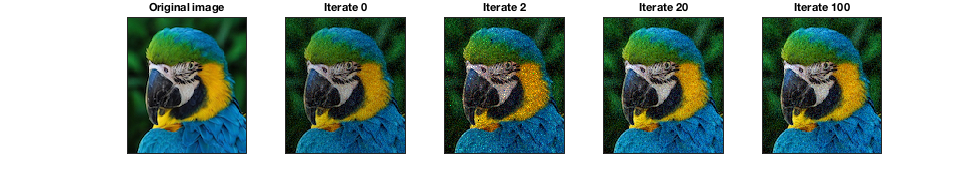
\includegraphics[scale=0.55]{parrot_signal_iterates} }
\hbox{\hspace{-1.7cm} 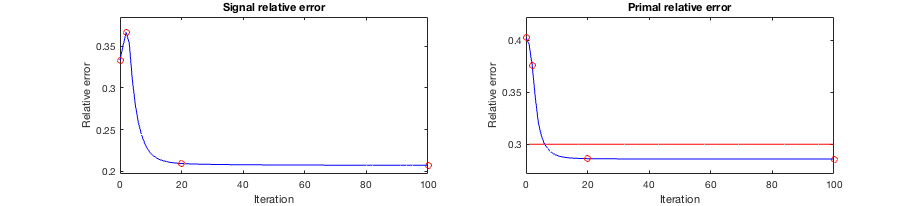
\includegraphics[scale=0.6]{parrot_signal_relative_error_2} }
\caption{Results from the GDD algorithm (Algorithm \ref{Alg:PGD}) applied to a test image separated into its three RGB channels.  Left: signal relative error $||xx^*- \mathbf{x}\mathbf{x}^*||_F / ||\mathbf{x}\mathbf{x}^*||_F$.  Right: primal relative error $||\caA(xx^*)-b||_2 /  ||b||_2$ with red line indicating primal feasibility.  Red circles denote the iterate signals pictured above.  Original signal is $128 \times 128$ pixels, with an oversampling of $L = 8$ and noise ratio $\epsilon_\rel = 0.30$.  Measurements use the mean of the three color channel values.}
\label{Fig:parrot_signal_relative_error_2}
\end{figure}
% experiments.figure.noisyimage_signal_relerr_various_saga_iterates

Figure \ref{Fig:parrot_signal_relative_error_2} demonstrates the tendency of the GDD algorithm to make significant progress during early iterates.  When the same set of models in Figure \ref{Fig:parrot_signal_relative_error_2} were solved with the wflow algorithm, the red channel converged to an infeasible solution (with primal residual $0.300068$), the green channel converged to a feasible solution (with primal residual $0.288473$), and the blue channel diverged.  





Table \ref{Tab:relative_errors_saga_vs_wflow} and Figure \ref{Fig:parrot_signal_relative_error_2} highlight the effectiveness of the GDD algorithm for noisy phase retrieval problems.  
The GDD algorithm is typically is more robust than the wflow algorithm and tends to recover signals successfully when there is minimal oversampling. 
Thus, among the phase retrieval models and methods considered in Chapter \ref{Sec:phase_retrieval} and this appendix, the PLGD model (\ref{Eqn:PLGD_ch2}) is the best suited for large-scale, unstructured noisy phase retrieval problems.

